\chapter{GIF++ Conditioning Tests}
\label{sec:rpc_gifpp_conditioning}

The conditioning tests of RPC gas gaps were performed at the GIF++
facility at CERN, which provides a controlled irradiation environment
to emulate the high-rate conditions expected at the HL-LHC. Several
RPC packages, comprising multiple gas gaps, were tested under
realistic operating conditions.

The conditioning procedure consists of gradually increasing the
applied high voltage in steps while continuously monitoring the gap
currents. At each voltage step, the detector response is allowed to
stabilise before proceeding to the next voltage level. In addition,
dedicated high-voltage scans are performed both before and after the
conditioning process to evaluate the evolution of the detector
behaviour. These scans are carried out under well-defined conditions,
including source-on and source-off configurations.

The evolution of the detector response during the conditioning
procedure is illustrated in Figure~\ref{fig:gifpp_conditioning_trend}.
The applied high voltage is increased in discrete steps, and the
corresponding gap currents exhibit stable plateaus at each voltage
level. Transient current increases are observed during voltage
ramping, which are consistent with the expected behaviour of RPC
detectors undergoing conditioning.

\begin{figure}[htbp]
    \centering
    \begin{subfigure}{0.48\textwidth}
        \centering
        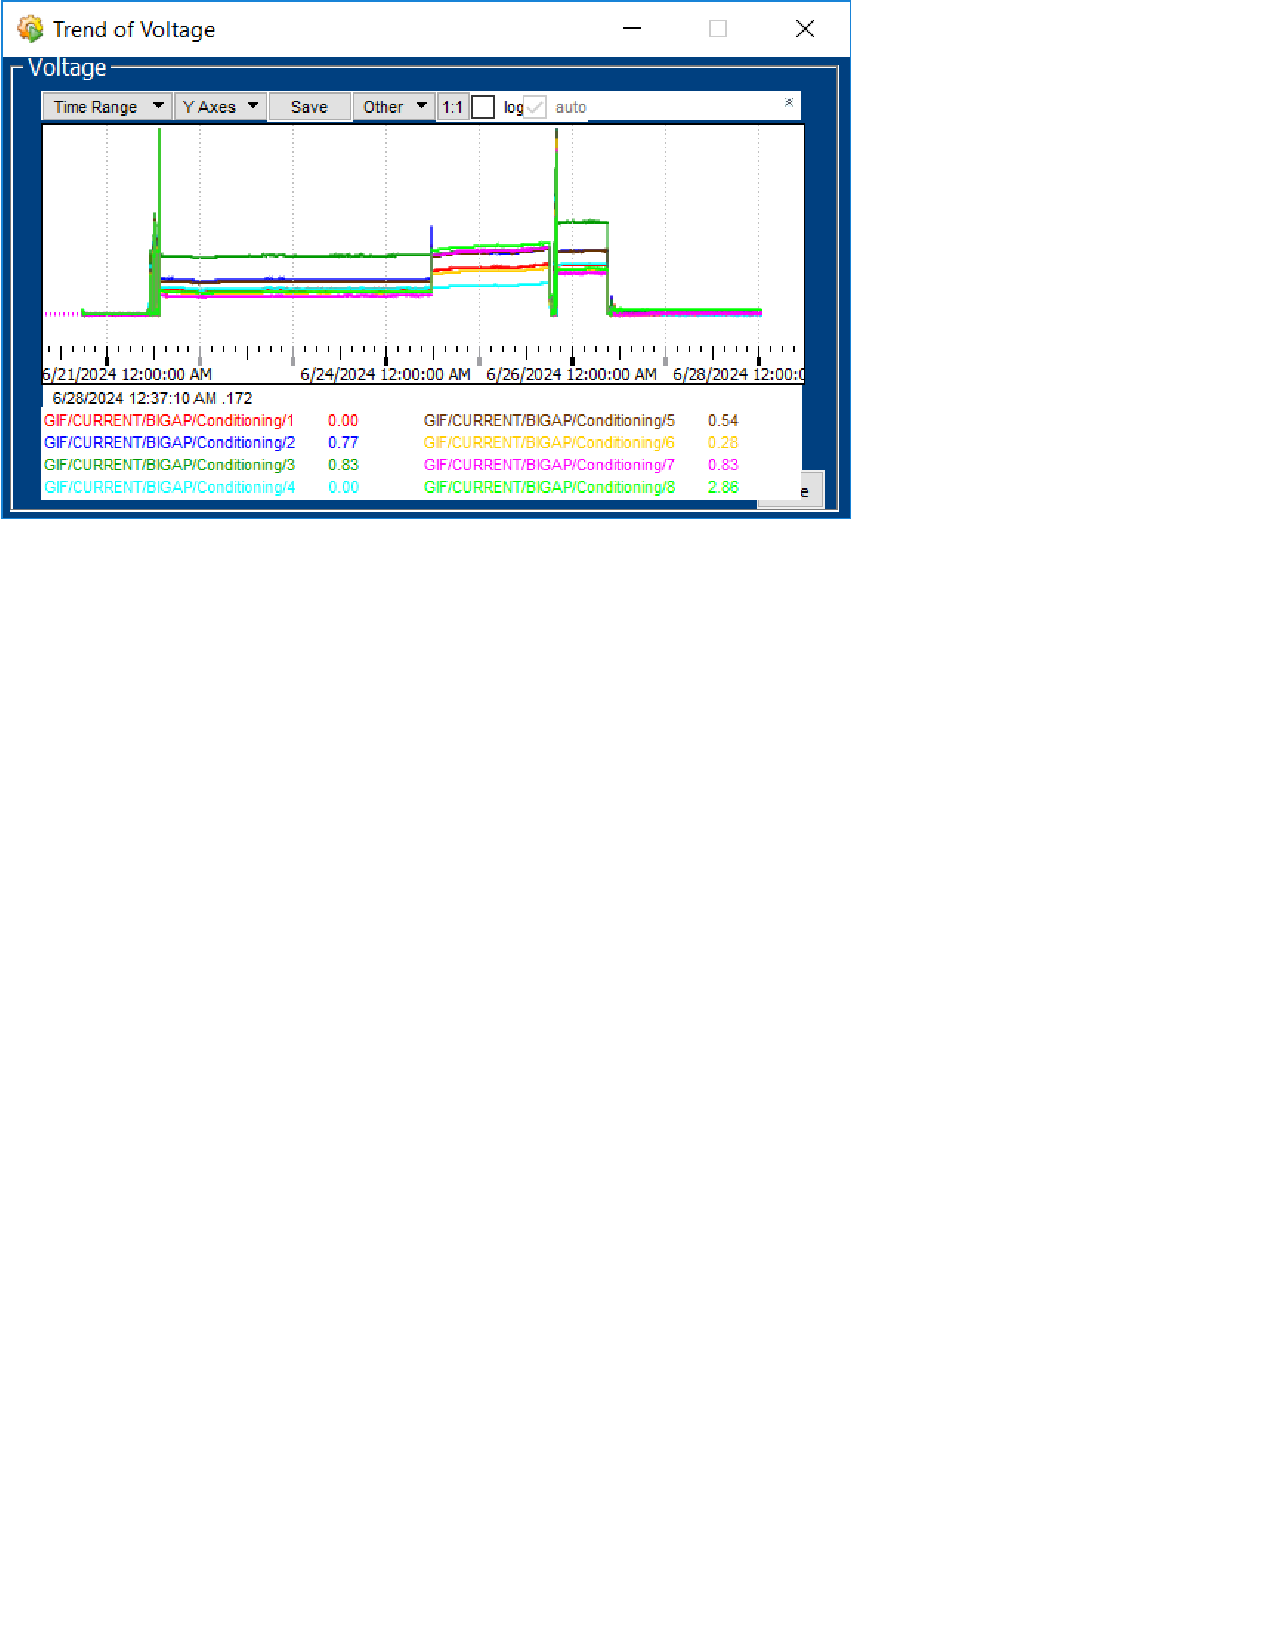
\includegraphics[width=\linewidth]{figures/RPC_main/V_trend_1.pdf}
        \caption{Voltage and current evolution (set A).}
    \end{subfigure}
    \hfill
    \begin{subfigure}{0.48\textwidth}
        \centering
        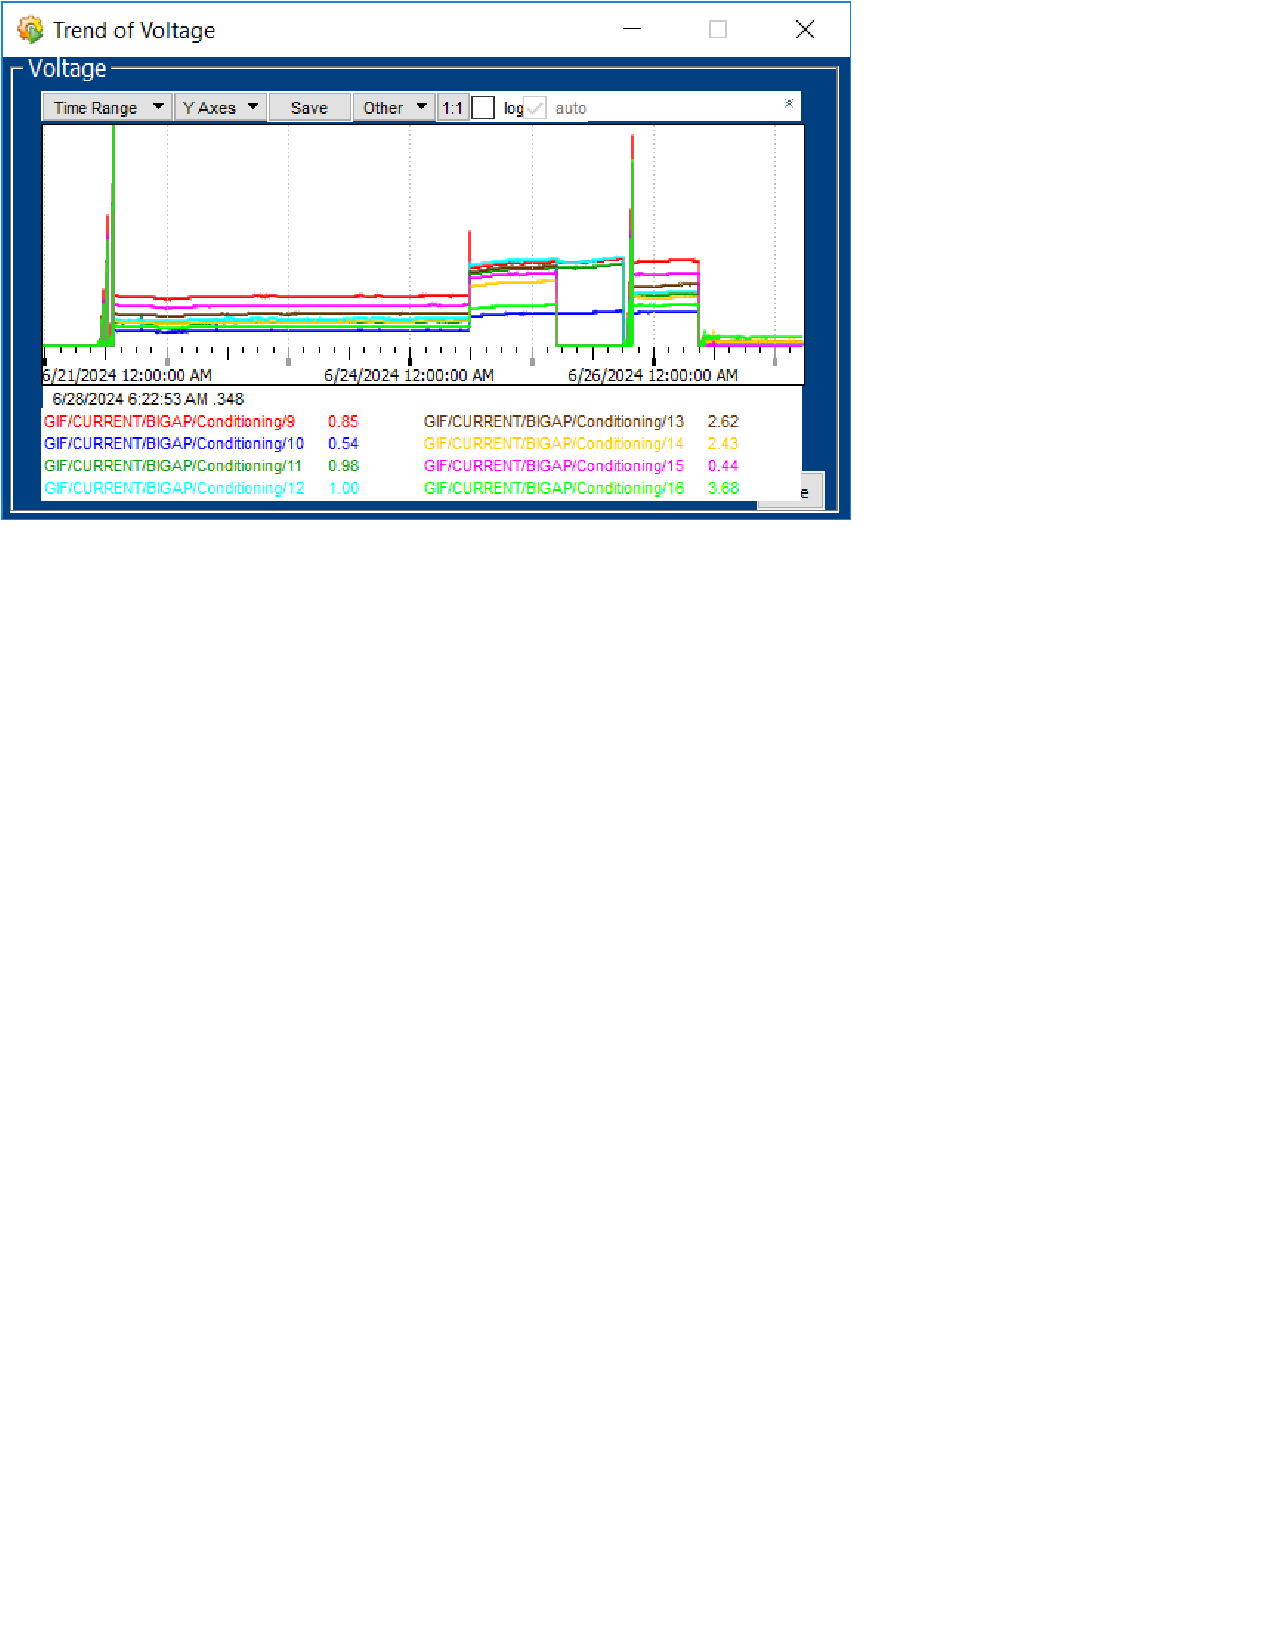
\includegraphics[width=\linewidth]{figures/RPC_main/V_trend_2.pdf}
        \caption{Voltage and current evolution (set B).}
    \end{subfigure}
    \caption{
    Evolution of high voltage and corresponding gap currents during the
    conditioning procedure at GIF++. Stable current plateaus are observed
    at each voltage step, indicating controlled detector behaviour.
    }
    \label{fig:gifpp_conditioning_trend}
\end{figure}

To quantify the impact of the conditioning, the initial and final
high-voltage scans are compared, as shown in
Figure~\ref{fig:gifpp_iv_comparison}. Each curve corresponds to an
individual RPC gas gap. A general reduction of the current is observed
after conditioning for most channels, indicating improved detector
stability. A small number of gas gaps exhibit increased current and
are subject to further investigation.

\begin{figure}[htbp]
    \centering
    \begin{subfigure}{0.48\textwidth}
        \centering
        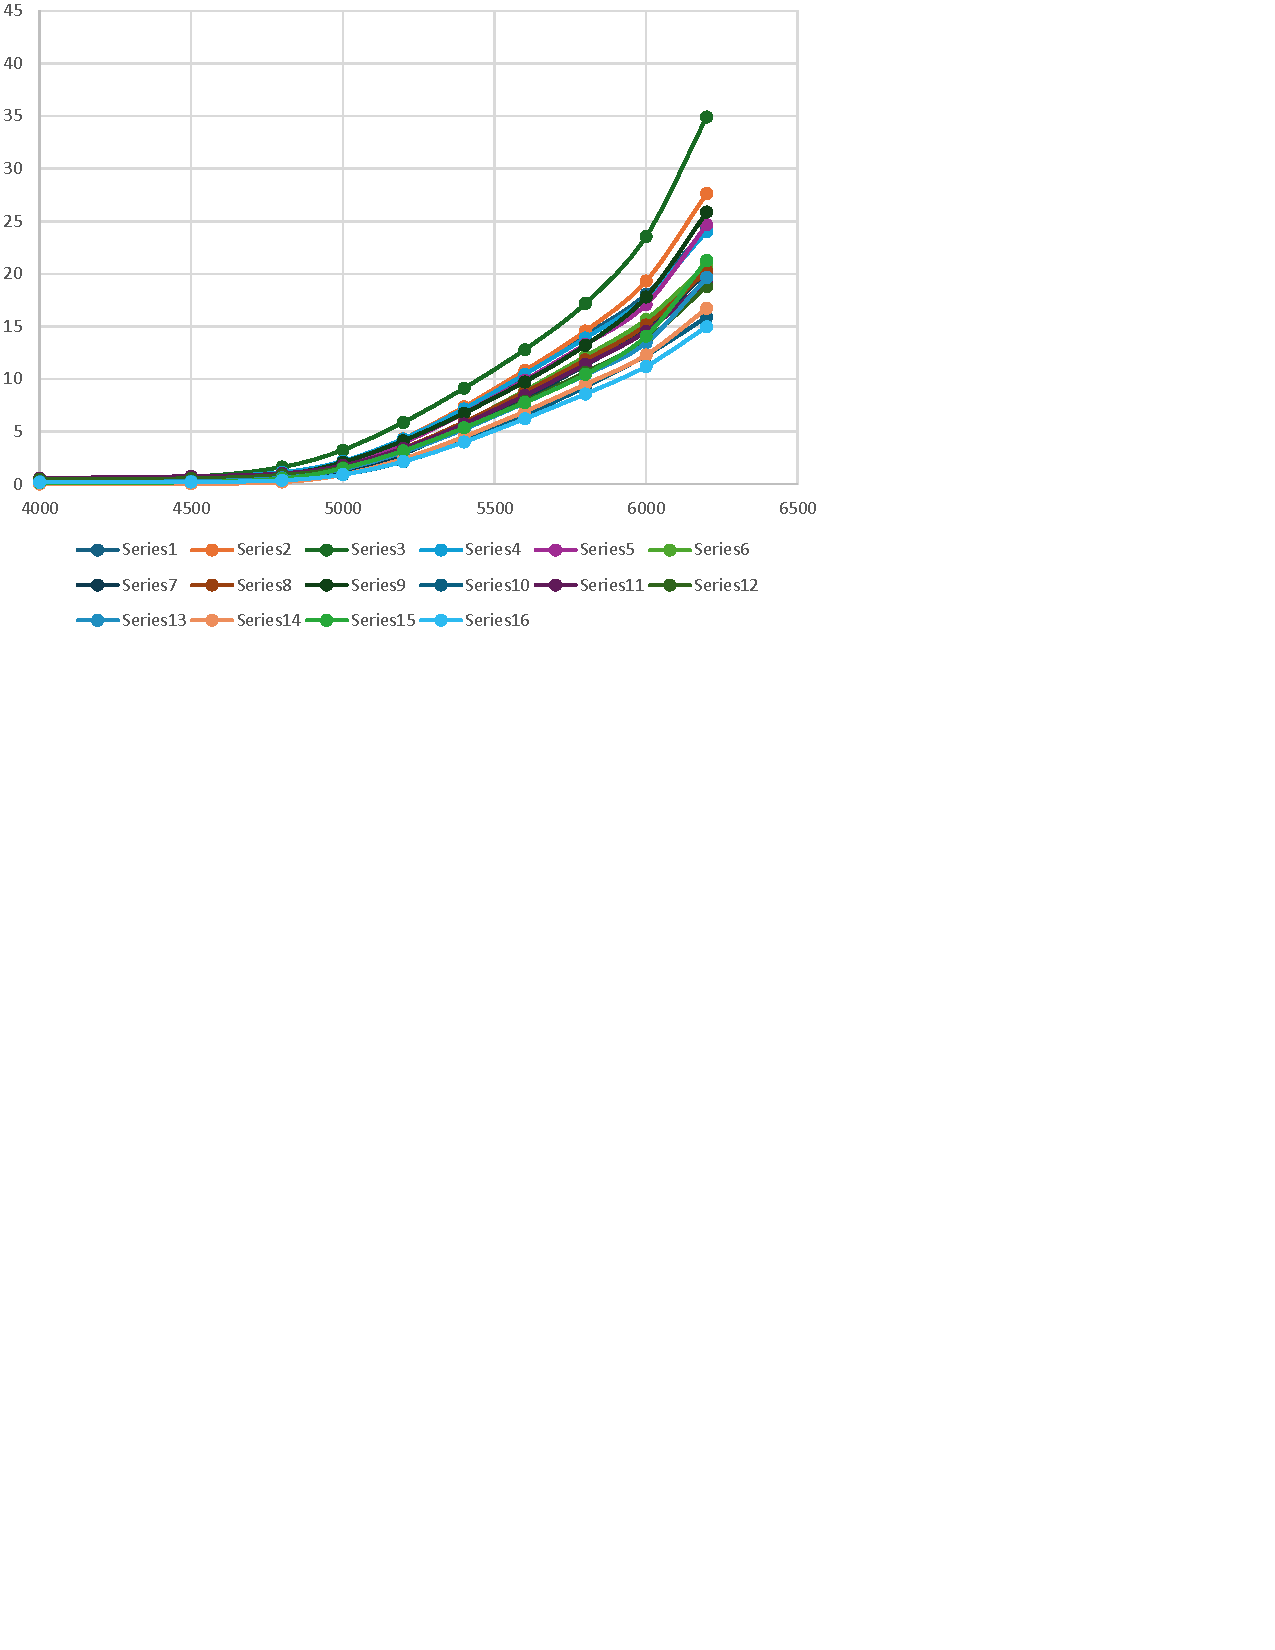
\includegraphics[width=\linewidth]{figures/RPC_main/Initial_scan.pdf}
        \caption{Initial high-voltage scan.}
    \end{subfigure}
    \hfill
    \begin{subfigure}{0.48\textwidth}
        \centering
        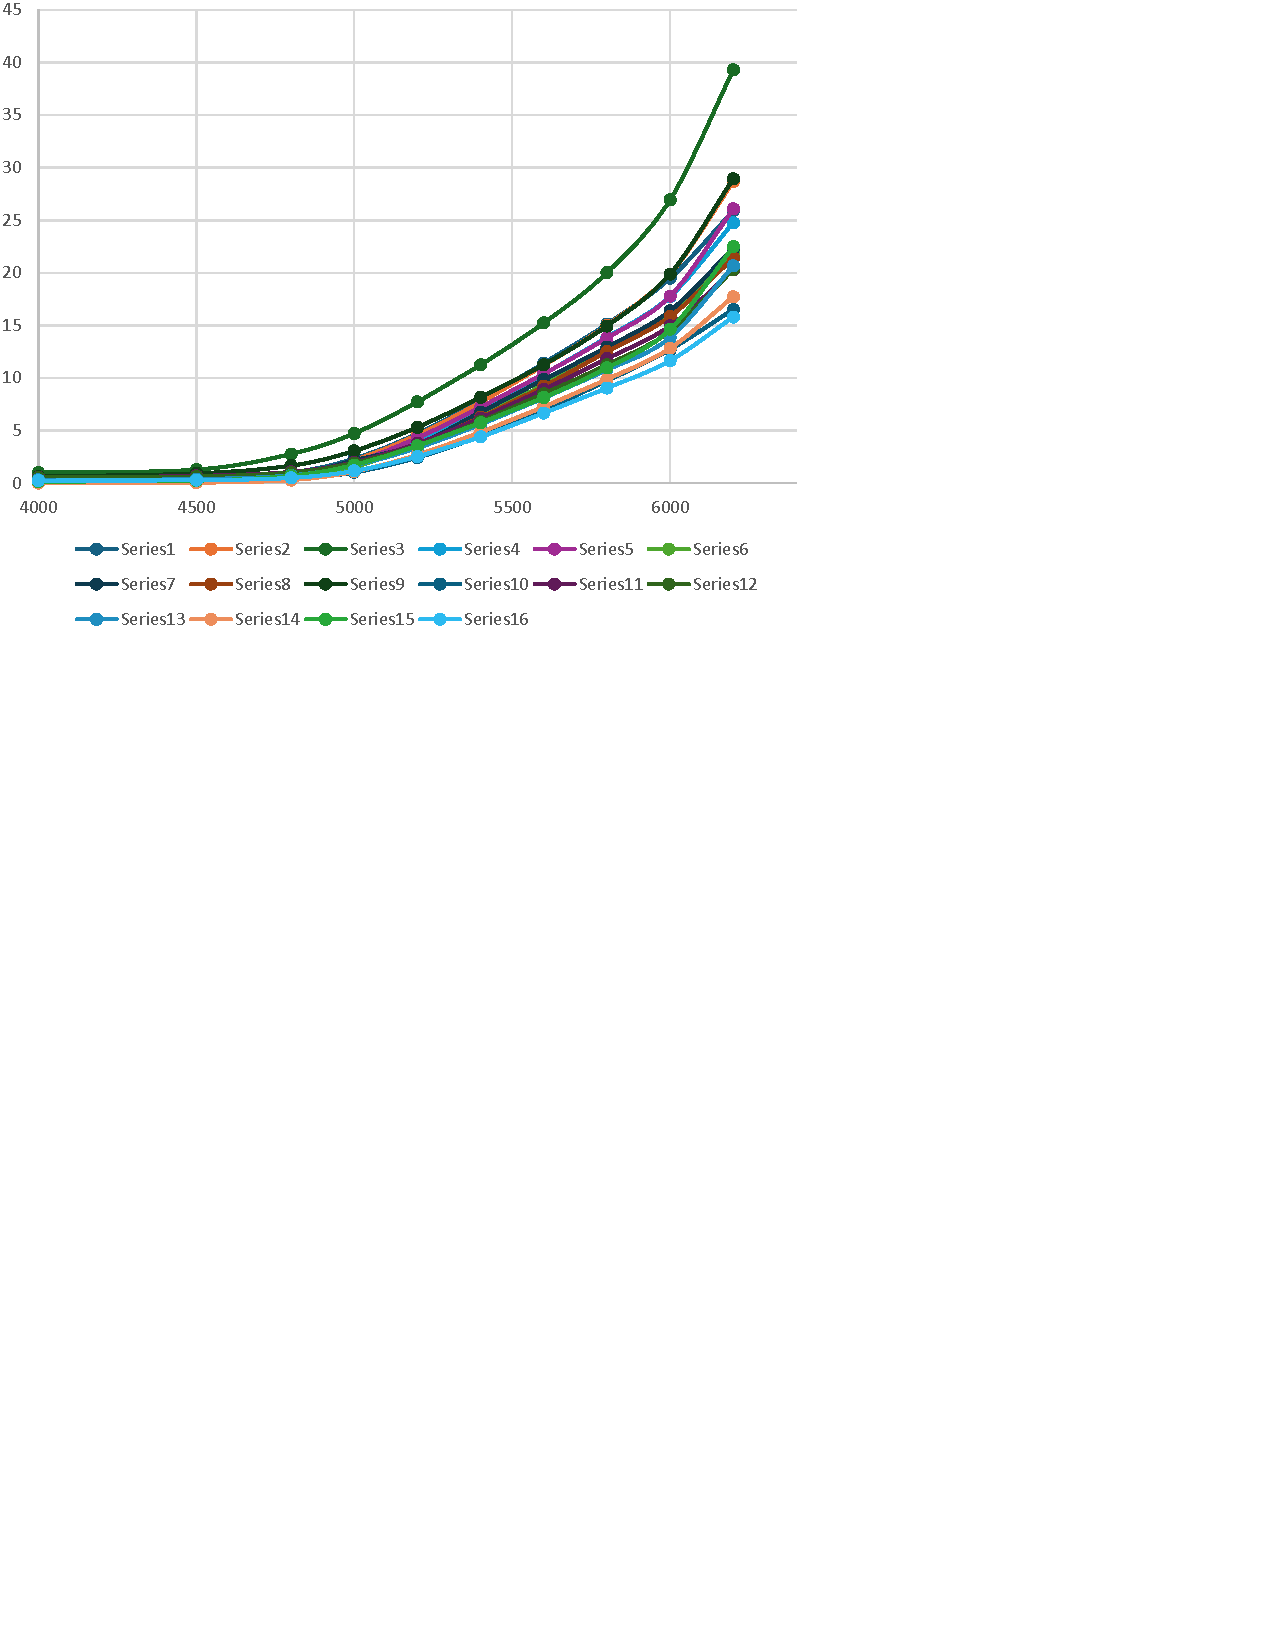
\includegraphics[width=\linewidth]{figures/RPC_main/Final_scan.pdf}
        \caption{Final high-voltage scan after conditioning.}
    \end{subfigure}

    \vspace{0.5cm}

    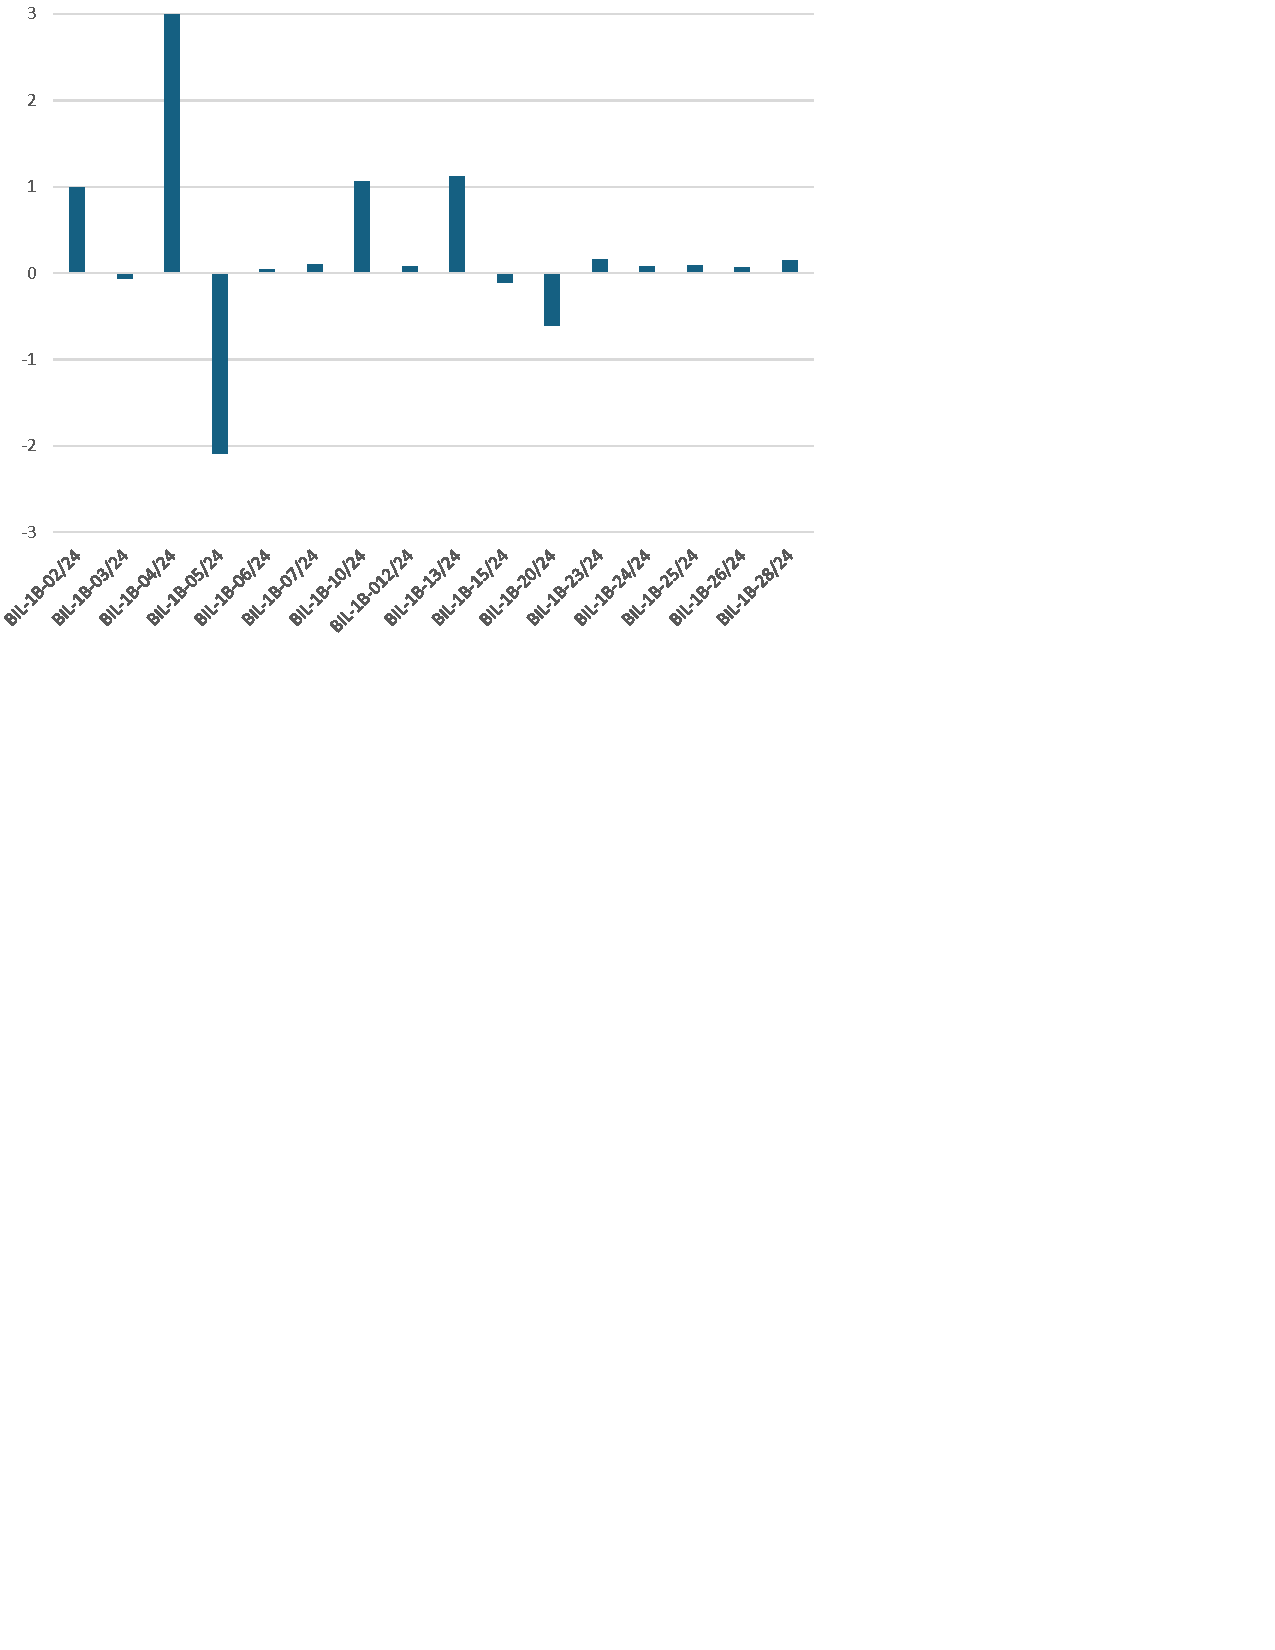
\includegraphics[width=0.6\textwidth]{figures/RPC_main/I_conparison_6000V.pdf}

    \caption{
    Comparison of RPC response before and after conditioning.
    Top: initial and final high-voltage scans for multiple gas gaps.
    Bottom: difference between final and initial currents evaluated at
    $6~\si{\kilo\volt}$, providing a direct measure of the conditioning
    effect. Negative values correspond to a reduction of current after
    conditioning. A general decrease of current is observed, indicating
    improved detector stability, while a small number of channels show
    deviations requiring further investigation.
    }
    \label{fig:gifpp_iv_comparison}
\end{figure}

Environmental conditions, such as atmospheric pressure variations,
are monitored during the tests and can affect the effective high
voltage. Their impact is found to be small and can be corrected for
in the analysis if needed. Overall, the results demonstrate that the
conditioning procedure leads to stable detector operation under
high-voltage and irradiation conditions representative of the
HL-LHC environment.